	\subsection{Abhören von verschlüsselter Kommuniktion bei bekannten Schlüsseln}
	% TODO@16.11.
	\subsubsection{1. Versuch - Im Networking Labor}
	Als praktisches Beispiel wird eine Testumgebung mit folgender Hardware aufgebaut
	\begin{itemize}
		\item 1x Switch
		\item 2x PC
		\item 1x Webserver
	\end{itemize}
	Dabei wird die Hardware nach folgendem Schema eingerichtet. Ein PC dient dabei als "BadGuy", der als 3. Person versucht
	die Kommunikation zwischen den zwei anderen Teilnehmern (PC und Webserver) zu entschlüsseln.
	\begin{figure}[H]
		\centering
		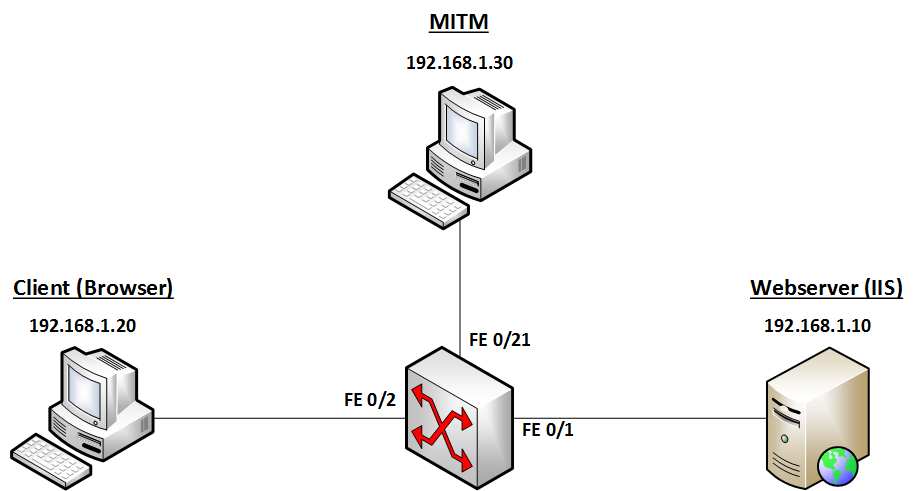
\includegraphics[width=.8\textwidth]{UebungsAufbau.png}
		\caption{Darstellung Versuchsaufbau}
		\label{fig:versuchsaufbau}
	\end{figure}
	Der Switch wird mit unten aufgeführten Befehlen so eingerichtet, dass auf dem Interface Fa0/21 ein Switchport Analyzer eingesetzt werden kann (siehe Exkurs \ref{sec:exkurs_span}).
	\commandbox{conf t}
	\commandbox{monitor session 1 source interface Fa0/1}
	\commandbox{monitor session 1 destination interface Fa0/21 encapsulation repliate}
	
	Der Versuch besteht aus 2 Teilversuchen. Im ersten Teilversuch wurde auf dem am SPAN Port angeschlossenen Rechner das Programm Wireshark gestartet ohne dabei die SSL Zertifikate auszutauschen. Das Ergebnis, ein gesnifftes TCP Paket auf dem Port 443 ist im Bild \ref{fig:ssl_encrypted_data} zu sehen.
	\begin{figure}[H]
		\centering
		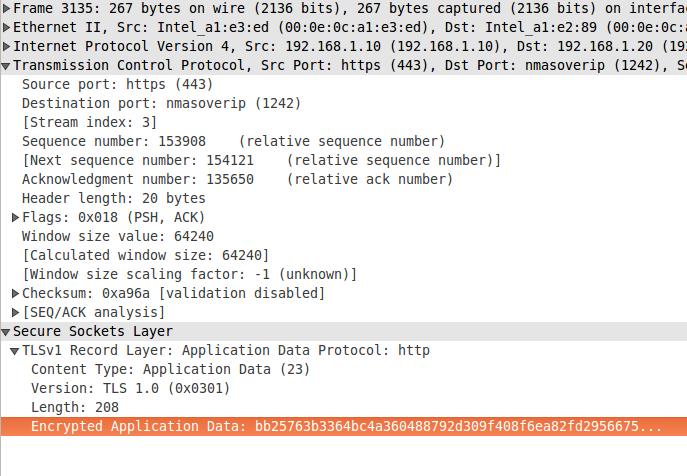
\includegraphics[width=.8\textwidth]{SSL_encrypted_data.png}
		\caption{Ansicht eines TCP Pakets mit SSL Verschlüsselung}
		\label{fig:ssl_encrypted_data}
	\end{figure}
	
	Beim zweiten Teilversuch wurde dem Wireshark der Schlüssel mitgeteilt. Über Settings unter Protokolle im Tab SSL wurde das Zertifikat 'unenc.pem' dem Wireshark SSL Protkoll zur Verfügung gestellt (siehe Bild \ref{fig:ssl_settings}).
	\begin{figure}[H]
		\centering
		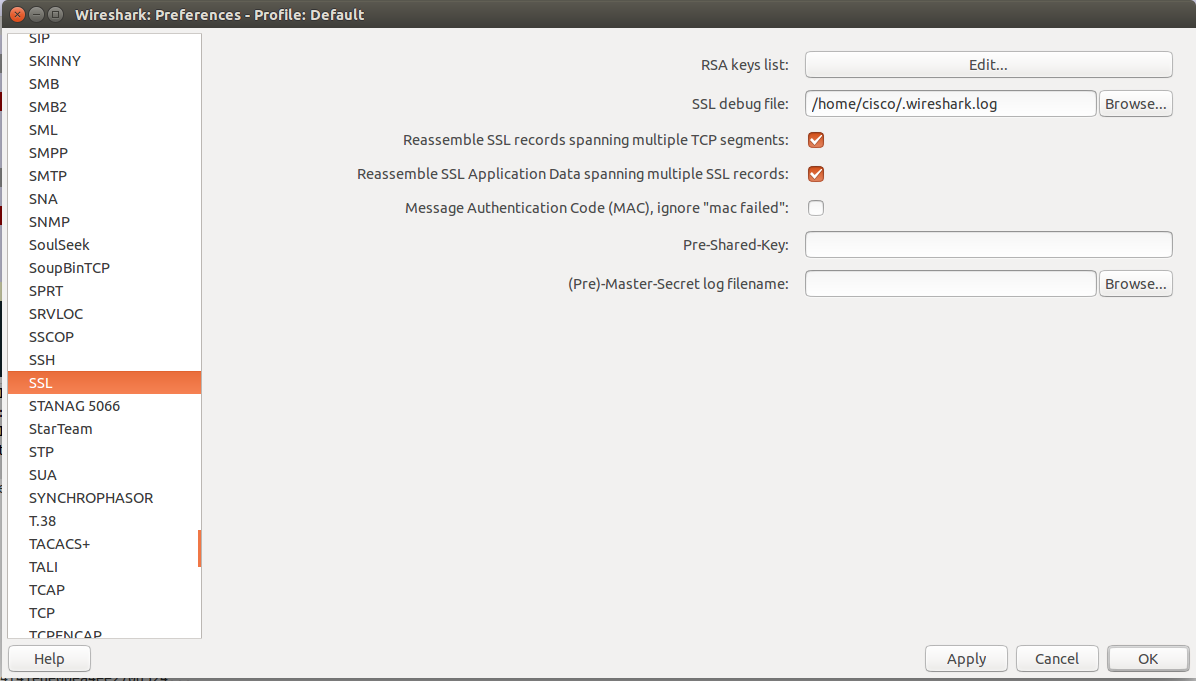
\includegraphics[width=.8\textwidth]{SSL_settings.png}
		\caption{Einstellungen für die SSL Key Übergabe}
		\label{fig:ssl_settings}
	\end{figure}
	Durch den Versuch wurde die Nachricht leider nicht lesbar entschlüsselt. Nach \citeA{wireshark} auf der Wireshark Website kann das Programm nur Schlüssel verwenden, welche nicht durch ein Passwort verschlüsselt sind. Da beim Versuch ein solcher Schlüssel verwendet wurde, musste der Schlüssel zuerst noch umgeformt werden.\\
	Zusätzlich kommt das Problem mit der Verschlüsselungsart hinzu. Auf dem Webserver findet ein Handshake mit der Diffie-Hellman Verschlüsselung statt und kann von Wireshark nicht entschlüsselt werden. Leider konnte der Webserver nicht umgeformt werden und dadurch wurde der 1. Versuch abgebrochen.\\
	%start des exkurs
	\shadebox{
		\subsection*{Exkurs: Switch Port Analyzer (SPAN)}\label{sec:exkurs_span}
		Switch Port Analyzer (kurz SPAN), oft auch port mirroring oder port monitoring genannt, kopiert Switch Netzwerkverkehr und sendet diesen an den SPAN Port zur Analyse durch einen Netzwerk Analyzer weiter. Durch Einschalten des SPAN, kann der Verkehr auf einem Switch überwacht werden durch Weiterleiten von eingehendem und ausgehendem Nachrichten an einen anderen Port [...] Netzwerk Analyzer können so zum Suchen von Fehlern von Netzwerkproblemen im Datenverkehr benutzt werden, ohne dass dabei das Netzwerk ausser Dienst genommen werden muss.\cite{span}
		}
	%ende des exkurs
	
	\subsubsection{2. Versuch - Über localhost}
	Da der 1. Versuch abgebrochen wurde, wurde ein 2. Versuch durchgeführt. Nach der Anleitung eines Entschlüsselungs Walkthrough der Wireshark Webseite \cite{wireshark} wurde dieser Versuch aufgebaut.
	\begin{enumerate}
		\item \textbf{Schlüssel und Zertifikat erzeugen}\\
		als erstes wurde ein RSA key und Zertifikat mit folgendem Befehl eingerichtet
		\commandbox{openssl req -new -x509 -out server.crt -nodes -keyout server.pem -subj /CN=localhost}
		\item \textbf{Server über localhost starten}
		\commandbox{openssl s\_server -www -cipher AES256-SHA -key server.pem -cert server.crt}
		\item \textbf{Schlüssel dem Tool übergeben}\\
		über die gleiche Einstellung wie bereits beim 1. Versuch wurde das server.pem Wireshark gegeben.
		\item \textbf{Capture und Analyse}\\
		Für Wireshark wurde ein Capturefilter auf TCP und Port 4433 eingesetzt. Danach wurde über die Konsole eine Serveranfrage gesendet.
		\commandbox{printf 'GET / HTTP/1.0' | openssl s\_client -ign\_eof}
		Das Capturing im Wireshark ist auf dem Bild \ref{fig:versuch_capture} zu sehen.
		\begin{figure}[H]
			\centering
			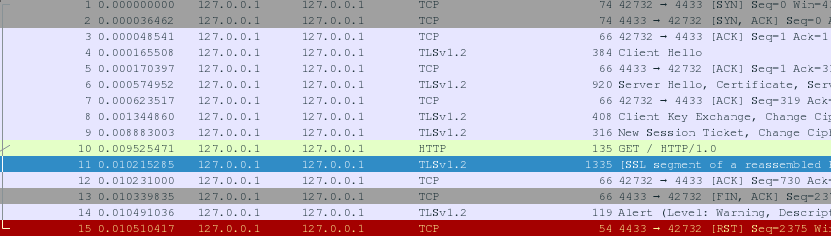
\includegraphics[width=\textwidth]{versuch_capture.png}
			\caption{Capture der Serveranfrage}
			\label{fig:versuch_capture}
		\end{figure}				
		Wenn man den TCP und SSL Stream ansieht, sieht man die jeweiligen Inhalte einmal verschlüsselt (Bild \ref{fig:tcp_stream}) und einmal unverschlüsselt (Bild \ref{fig:ssl_stream}).
		\begin{figure}[H]
			\centering
			\begin{subfigure}{.4\textwidth}
				\centering
				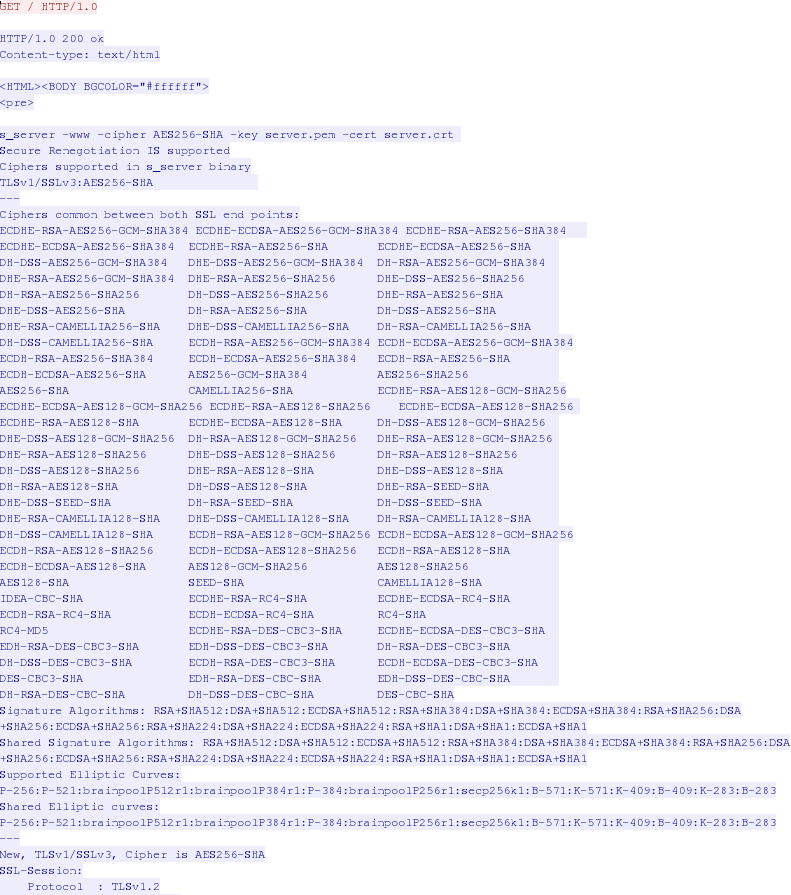
\includegraphics[width=\linewidth]{versuch_ssl_stream.png}
				\caption{entschlüsselter Datenstrom}
				\label{fig:ssl_stream}
			\end{subfigure}
			\begin{subfigure}{.4\textwidth}
			 	\centering
				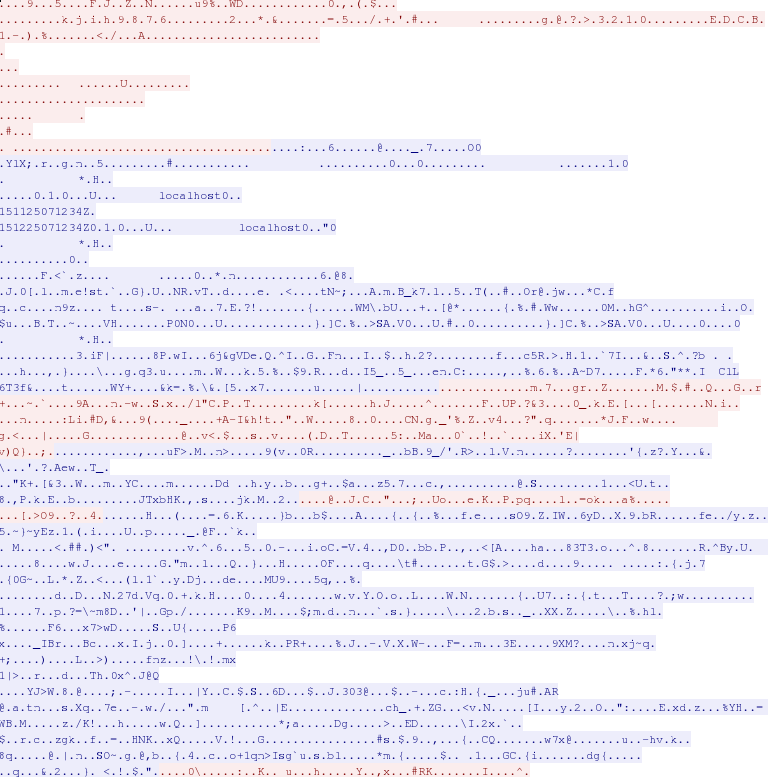
\includegraphics[width=\linewidth]{versuch_tcp_stream.png}
				\caption{verschlüsselter Datenstrom}
				\label{fig:tcp_stream}
			\end{subfigure}
			\caption{Paketanalyse im Wireshark}
		\end{figure}
	\end{enumerate}
	
	\subsubsection{Versuchsergebnisse}
	Mit Wireshark ist das Auslesen von verschlüsselten Paketen kein Problem, solange der Schlüssel bekannt und dieser denn Bedingungen zum Entschlüsseln entspricht. Ein solcher Schlüssel darf nicht mit einem Password selbst verschlüsselt sein und darf nicht mit dem Diffie-Hellman Verfahren gemacht worden sein.\\
	Werden diese Bedingungen erfüllt, erscheinen alle Pakete im Klartext. 
	
	\subsection{Analyse von bereits vorhandenen Tools} % keine Enterprise-lösungen
	\begin{description}
		\item[Wireshark] Ein Tool zur Analyse des Netzwerkverkehrs. Kann eine Vielzahl von Protokollen analysieren und bei gegebenem Schlüssel sogar entschlüsseln.
		\item[Vault] Ein Opensource Tool zum Speichern von Tokens auf einem Server. Durch eine Konfiguration kann der Speicherort angegeben werden. Das Tool hat die Möglichkeit eine hohe Verfügbarkeit durch Multi-Server Mode herzustellen.\\
		Tokens können so jederzeit online abgerufen werden.
		\item[KeyBox] Eine Opensource web-based ssh Konsole für zentralisierte Administration von Systemzugriffen auf mehrere Systeme.
		\item[privacyID3A] Ist ein webbasiertes Tool, das als Authentifizierungssystem von Benutzern verwendet werden kann. Es bietet eine vielzahl an möglichen Authentifizierungen und kann durch einen Administrator zentral verwaltet werden. Der Administrator und Benutzer können sich jeweils auf das Benutzersystem einloggen.
	\end{description}